\section{STM32F411CEU6}
\subsection{Why this MCU?}
Our choice of the STM32F411CEU6 stems from a commitment to innovation, steering away from the common trend of utilizing a Pi Zero, a path often trodden by other groups. Delving into the intricacies of our decision, let's explore the schematic in \autoref{fig:Blackpill_STM32F411CEU6_Schematic}.
\begin{figure}[H]
    \centering
    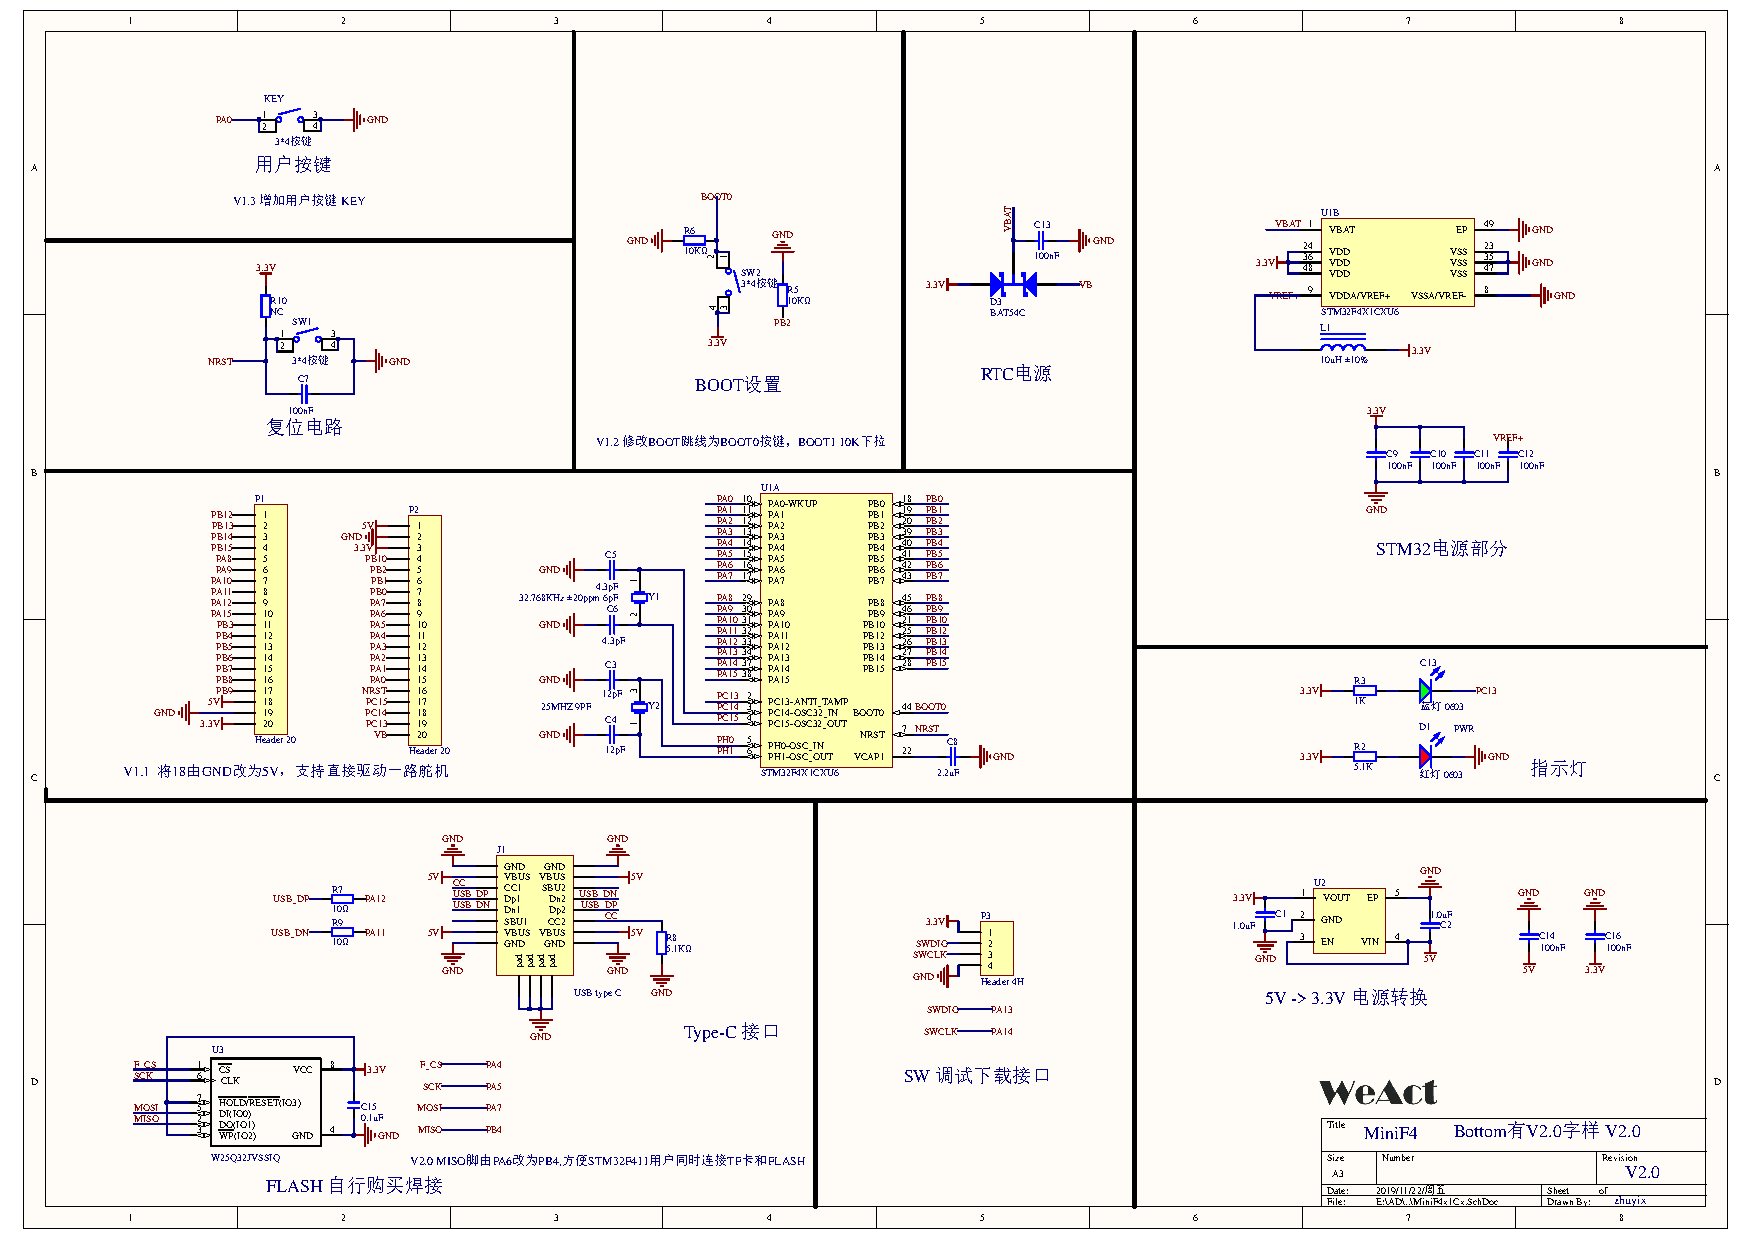
\includegraphics[width=1\linewidth]{img//blackpill/original-schematic-STM32F411CEU6_WeAct_Black_Pill_V2.0.pdf}
    \caption{Blackpill STM32F411CEU6 Schematic}
    \label{fig:Blackpill_STM32F411CEU6_Schematic}
\end{figure}
\begin{itemize}
    \item \textbf{Circuit with Buttons:} The schematic reveals a carefully designed circuit accommodating essential buttons - Key, Switch, and Boot - crucial for operational control.

    \item \textbf{Real-Time Clock (RTC):} A dedicated circuit for real-time clock functionality ensures precise timing and synchronization within our motor control system.

    \item \textbf{STM32F411CEU6 Pinout:} The MCU itself is dissected with a pinout, providing insights into the connections and functionalities of each pin.

    \item \textbf{Flash Circuit:} A specialized flash circuit, integral for storing and retrieving data, contributes to the robust performance of our system.

    \item \textbf{Voltage Regulator:} The presence of a voltage regulator ensures stable and reliable power distribution throughout the system.

    \item \textbf{Additional Circuits:} Beyond these components, the schematic highlights several other circuits vital for the holistic functionality of our design.
\end{itemize}

Moving from the abstract schematic to the tangible layout, the dimensions in \autoref{fig:Blackpill_STM32F411CEU6_Dimensions} depict the spatial arrangement of each component. Assembled into a cohesive unit, the complete PCB with the integrated STM32F411CEU6 is visualized in \autoref{fig:Blackpill_STM32F411CEU6_Picture}.
\begin{figure}[H]
    \centering
    \begin{subfigure}{0.48\textwidth}
        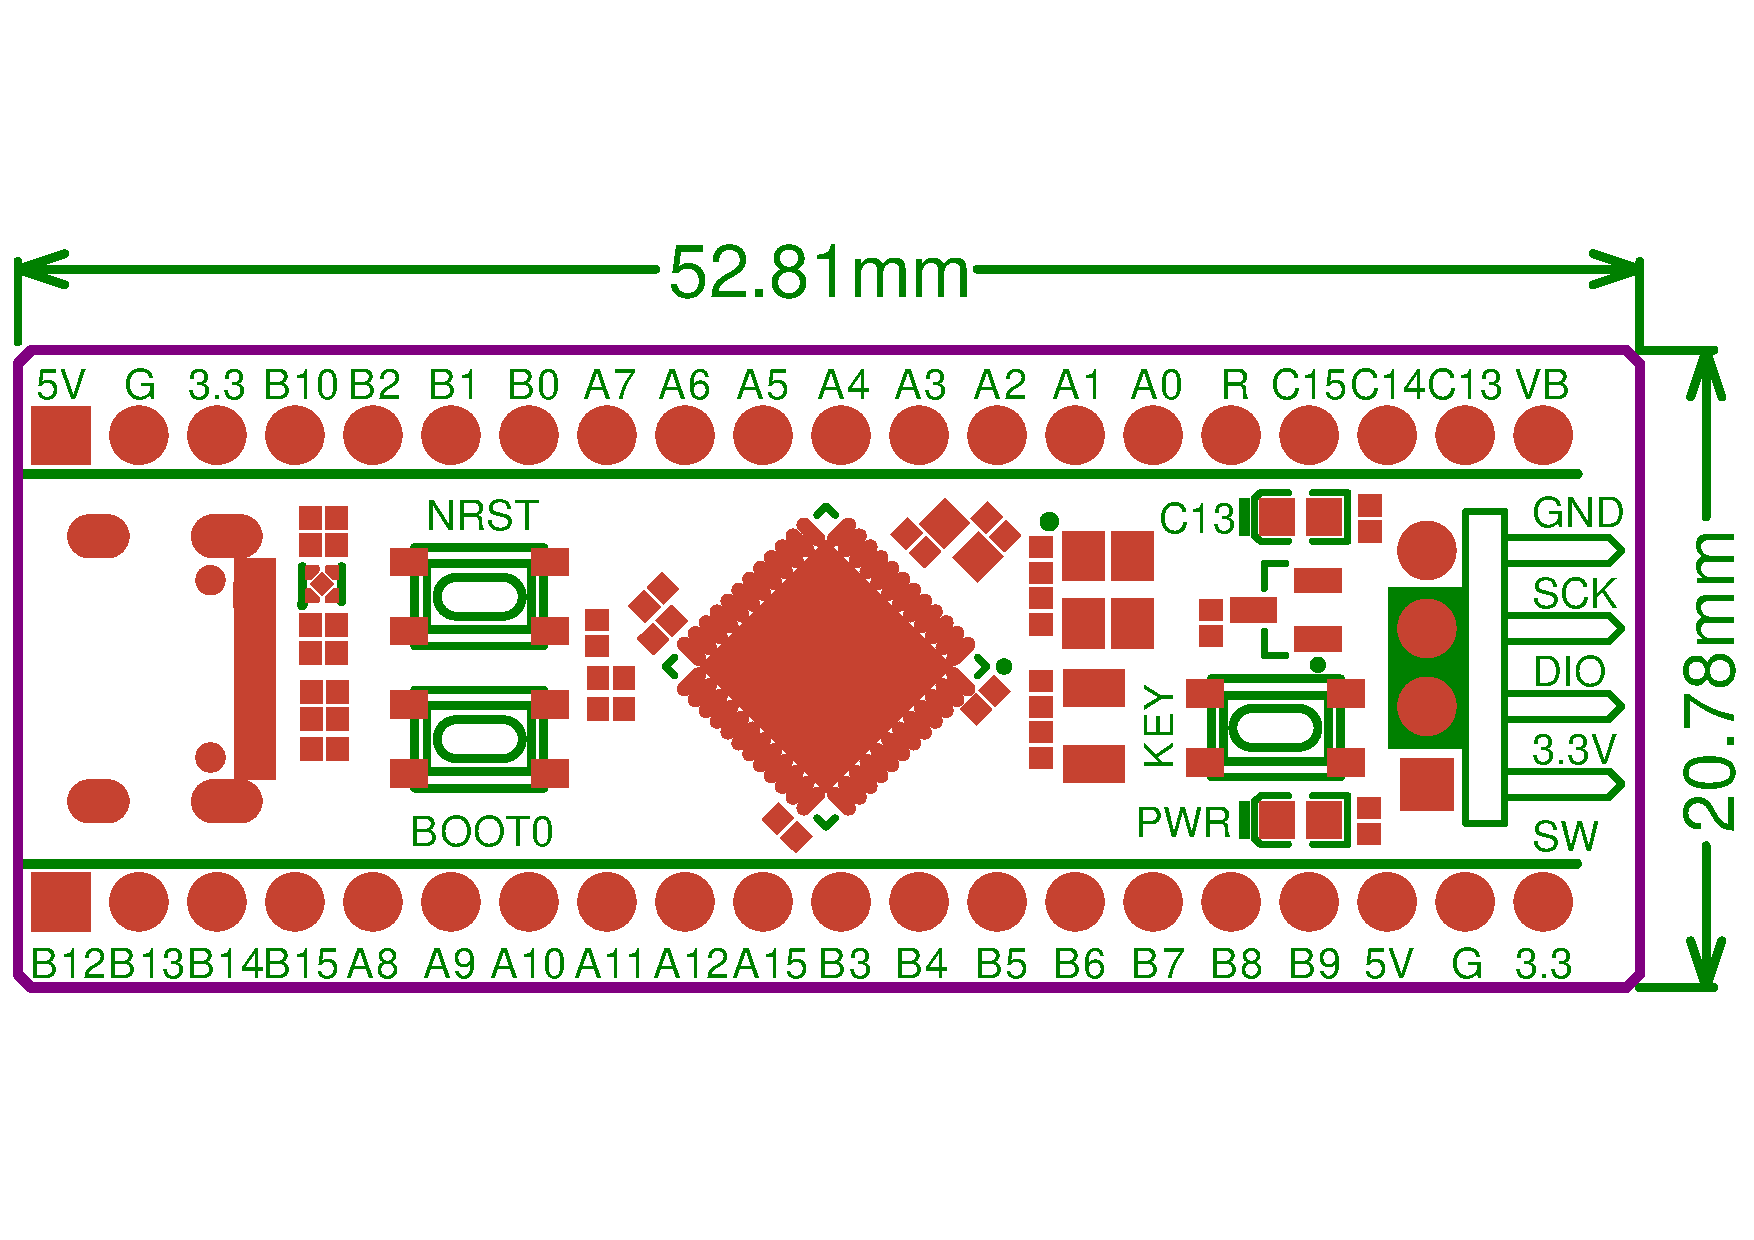
\includegraphics[width=\linewidth]{img/blackpill/original-dimensions-STM32F411CEU6_WeAct_Black_Pill_V2.0.pdf}
        \caption{Blackpill STM32F411CEU6 Dimensions}
        \label{fig:Blackpill_STM32F411CEU6_Dimensions}
    \end{subfigure}
    \hfill
    \begin{subfigure}{0.48\textwidth}
        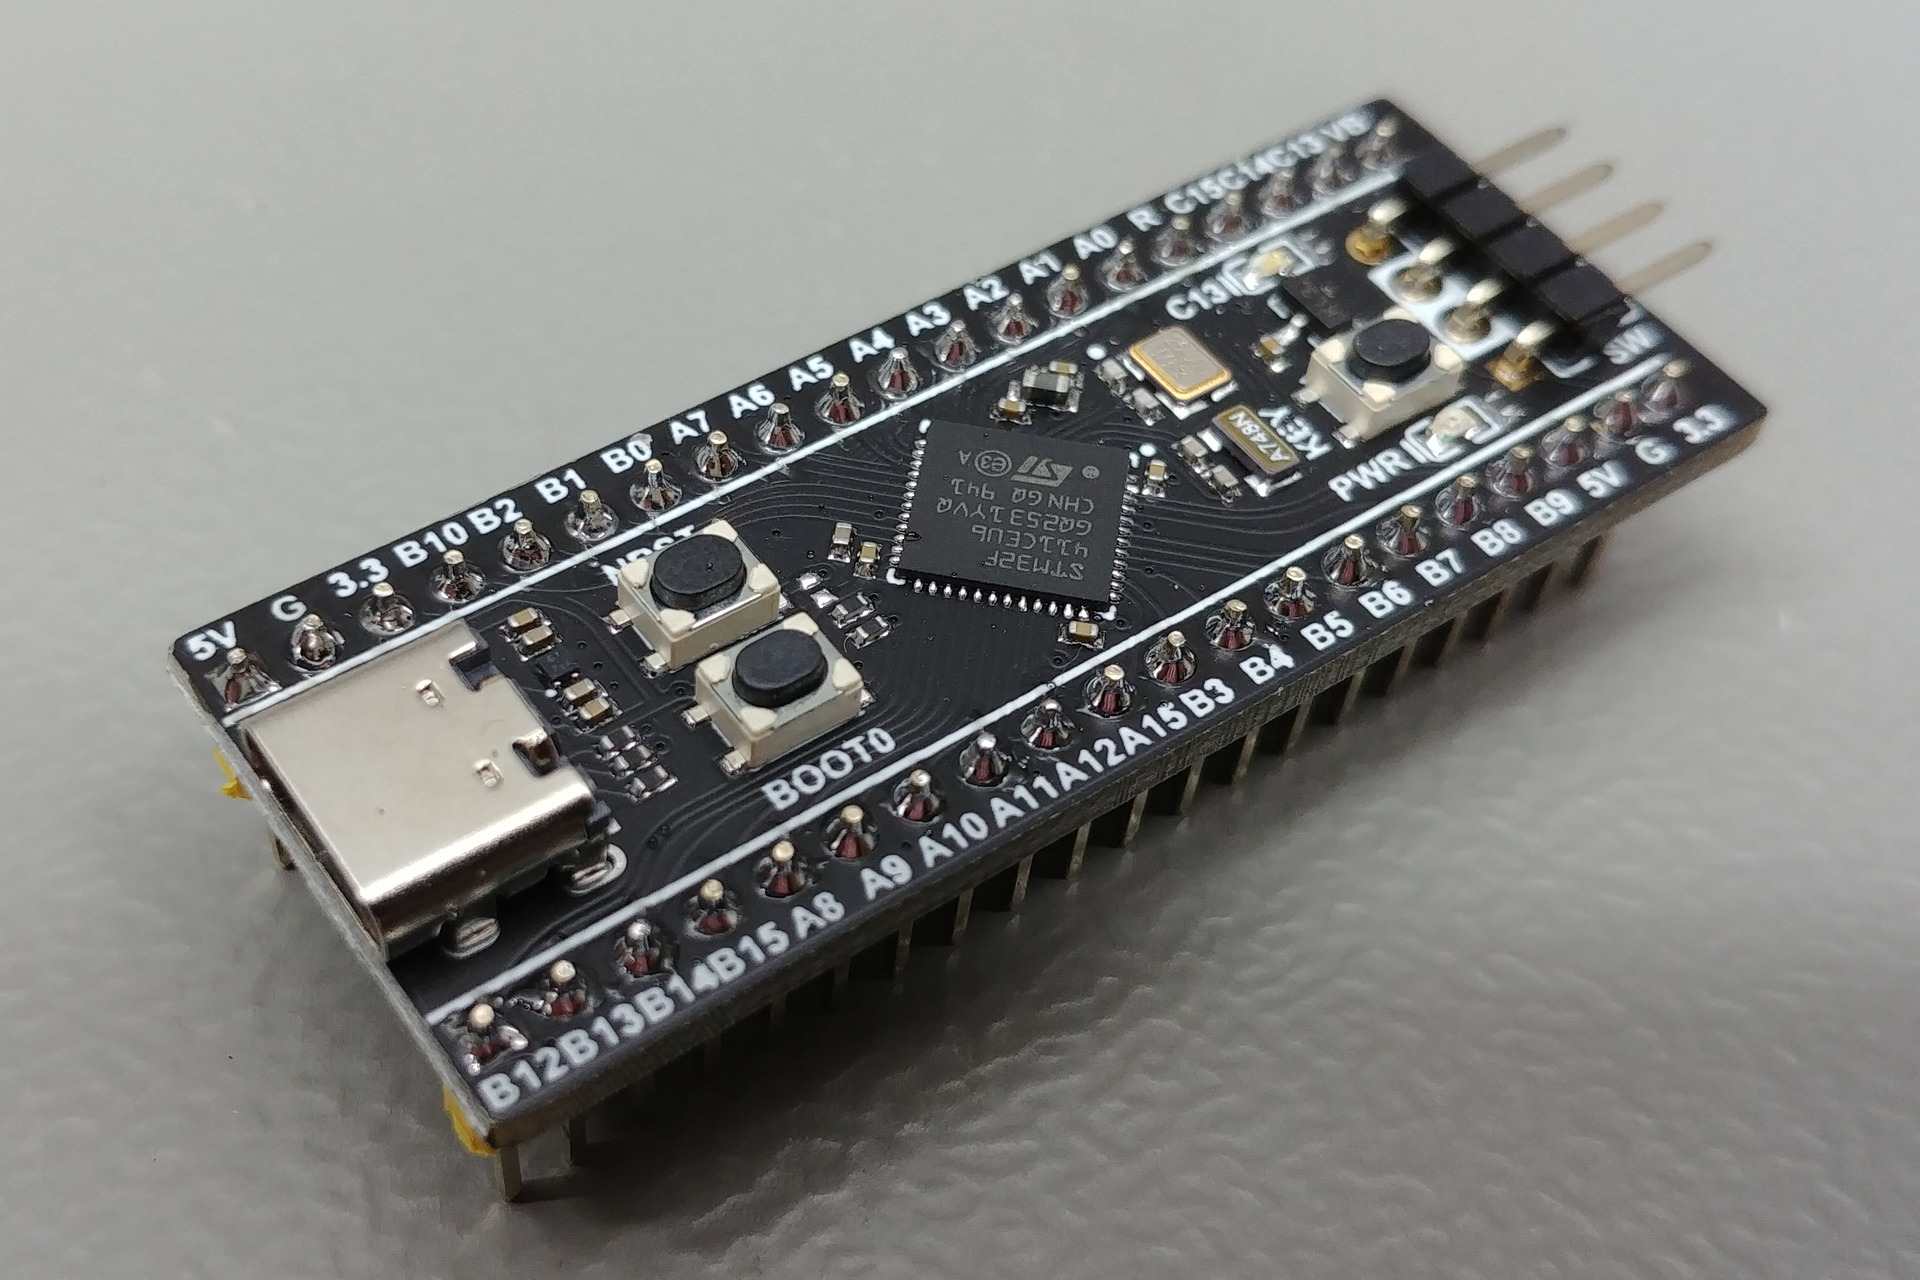
\includegraphics[width=\linewidth]{img/blackpill/STM32F411CEU6_WeAct_Black_Pill_V2.0-1.jpg}
    \caption{Blackpill STM32F411CEU6 Picture}
    \label{fig:Blackpill_STM32F411CEU6_Picture}
    \end{subfigure}
\end{figure}

\subsection{Specifications}
    \subsubsection{Microcontroller:}
    \begin{itemize}
        \item Part: STM32F411CEU6
        \item Manufacturer: ST-Microelectronics
        \item Core: Arm Cortex-M4
        \item Max. Clock Speed: 100MHz
        \item Package: UFQFPN 48 pins
    \end{itemize}

    \subsubsection{Internal Memories:}
    \begin{itemize}
        \item FLASH: 512KiB
        \item SRAM: 128KiB
    \end{itemize}

    \subsubsection{Oscillators:}
    \begin{itemize}
        \item HSI: 16MHz
        \item HSE: 25MHz (Critical for precise motor control)
        \item LSI: 32kHz
        \item LSE: 32.768kHz
    \end{itemize}

    \subsubsection{Power:}
    \begin{itemize}
        \item Voltage Input: +3.52V to +5.25V
        \item Power Sources: Any +3.3V pin, Any +5V pin, USB connector
        \item Backup battery: Supported
    \end{itemize}

    \subsubsection{Regulator:}
    \begin{itemize}
        \item Manufacturer: Diodes Incorporated
        \item Part: AP7343 (6T)
        \item Input: +3.52V to +5.25V
        \item Output: +3.3V @ 300mA
    \end{itemize}

    \subsubsection{PCB:}
    \begin{itemize}
        \item Color: Black
        \item Size (w x l): 20.78mm x 52.81mm
        \item Mounting: Breadboard
    \end{itemize}

    \subsubsection{Inputs \& Outputs:}
    \begin{itemize}
        \item Reset button (Active low)
        \item BOOT0 button (Active high)
        \item User button (Active low)
        \item Power LED (Connected to +3.3V rail)
        \item User LED (Connected to PC13)
    \end{itemize}

    \subsubsection{Connectors \& Headers:}
    \begin{itemize}
        \item Header 1 (20x1, male): 5V, GND, 3.3V, Motor Control Pins (PB0-PB10, PA0-PA7, PC13, NRST, PC15, PC14, VBAT)
        \item Header 2 (20x1, male): Motor Control Pins (PB12-PB15, PA8-PA15, PB3-PB9, 5V, GND, 3.3V)
        \item USB Connector (USB C): VBUS, D-, D+, GND (For potential external communication)
        \item SWD Header (4x1, male): 3.3V, SWDIO (PA13), SWCLK (PA14), GND (For debugging and programming)
    \end{itemize}

    \subsubsection{Devices:}
    \begin{itemize}
        \item Generic EEPROM (I2C): SOP 8 pins, Generic I2C EEPROM
        \item Connected to PA4 (CS), PB4 (DO), +3.3V rail (WP, HOLD), Ground plane (GND), PA7 (DI), PA5 (CLK), +3.3V rail (VCC)
    \end{itemize}

All information from this section has been retrieved thru these sources \cite{stm32datasheet,stm32base,stmicro}.